\newpage
\section{Resoconto verifica documenti}

In questa sezione del documento vengono descritti e analizzati gli esiti delle attività di verifica svolte su tutti i documenti che vengono consegnati nelle varie revisioni di avanzamento del progetto.
L’analisi dei documenti mediante la tecnica \textit{Walkthrough} ha reso possibile individuare alcuni errori frequenti, che si sono aggiunti alla lista di controllo stilata ed aggiornata nelle varie revisioni, utile per applicare la tecnica \textit{Inspection} nelle future attività di verifica.\\
Il team, attraverso il software interno \textit{NetBreakDB}, è riuscito ad effettuare i tracciamenti per le componenti di interesse previste da ogni revisione (casi d’uso-requisiti, requisiti-fonti, requisiti-componenti, requisiti-classi, etc.).\\
Inoltre, questo software è stato utilizzato per generare le tabelle dei vari test e dei relativi tracciamenti con requisiti, componenti, classi e metodi.
	
	\subsection{Revisione dei Requisiti}
	Di seguito, sono riportati gli esiti delle verifiche sottoposte a tutti i documenti, per il calcolo della metrica \textit{Indice Gulpease} (\hyperlink{MPC19}{MPC19}).
	
		\begin{longtable}{|>{\centering\arraybackslash}p{5.5cm}|>{\centering\arraybackslash}p{5cm} | >{\centering\arraybackslash}p{5cm}|}
			\hline
			\rowcolor{Gray}
			\textbf{Documento} & \textbf{Indice Gulpease} & \textbf{Esito} \\
			\hline
			\textit{\NdP\ 1.0.0} & 49 & \textcolor{Green}{\textit{Superato}}\\
			\hline
			\textit{\PdP\ 1.0.0} & 50 & \textcolor{Green}{\textit{Superato}} \\
			\hline
			\textit{\PdQ\ 1.0.0} & 42 & \textcolor{Green}{\textit{Superato}}\\
			\hline
			\textit{\AdR\ 1.0.0} & 68 & \textcolor{Green}{\textit{Superato}} \\
			\hline
			\textit{\SdF\ 1.0.0} & 54 & \textcolor{Green}{\textit{Superato}}\\
			\hline
			\textit{\G\ 1.0.0}& 43 & \textcolor{Green}{\textit{Superato}}\\
			\hline
			\textit{Verbale Interno - 28/11/2016}		& 	60	&	\textcolor{Green}{\textit{Superato}}	\\
			\hline
			\textit{Verbale Interno - 01/12/2016}		& 	63	&	\textcolor{Green}{\textit{Superato}}	\\
			\hline
			\textit{Verbale Interno - 12/12/2016}		& 	61	&	\textcolor{Green}{\textit{Superato}}	\\
			\hline
			\textit{Verbale Esterno - 22/12/2016}		& 	59	&	\textcolor{Green}{\textit{Superato}}	\\
			\hline
			\textit{Verbale Interno - 28/12/2016}		& 	61	&	\textcolor{Green}{\textit{Superato}}	\\
			\hline
		
		\caption{Resoconto verifiche documenti - RR}
	\end{longtable}

\newpage	
	\subsection{Revisione di Progettazione}
	Di seguito, sono riportati gli esiti delle verifiche sottoposte a tutti i documenti, per il calcolo della metrica \textit{Indice Gulpease} (\hyperlink{MPC19}{MPC19}).
	
			\begin{longtable}{|>{\centering\arraybackslash}p{5.5cm}|>{\centering\arraybackslash}p{5cm} | >{\centering\arraybackslash}p{5cm}|}
				\hline
				\rowcolor{Gray}
				\textbf{Documento} & \textbf{Indice Gulpease} & \textbf{Esito} \\
				\hline
				\textit{\ST\ 1.0.0} & 67  & \textcolor{Green}{\textit{Superato}}\\
				\hline
				\textit{\NdP\ 2.0.0} & 57  & \textcolor{Green}{\textit{Superato}}\\
				\hline
				\textit{\PdP\ 2.0.0} & 55 & \textcolor{Green}{\textit{Superato}} \\
				\hline
				\textit{\PdQ\ 2.0.0} & 54  & \textcolor{Green}{\textit{Superato}}\\
				\hline
				\textit{\AdR\ 2.0.0} & 70  & \textcolor{Green}{\textit{Superato}} \\
				\hline
				\textit{\G\ 2.0.0}& 49 & \textcolor{Green}{\textit{Superato}}\\
				\hline
				\textit{Verbale Interno - 27/01/2017}		& 	55	&	\textcolor{Green}{\textit{Superato}}	\\
				\hline
				\textit{Verbale Interno - 04/02/2017}		& 	64	&	\textcolor{Green}{\textit{Superato}}	\\
				\hline
				\textit{Verbale Interno - 13/02/2017}		& 	58	&	\textcolor{Green}{\textit{Superato}}	\\
				\hline
				\textit{Verbale Esterno - 16/02/2017}		& 	60	&	\textcolor{Green}{\textit{Superato}}	\\
				\hline
				\textit{Verbale Interno - 17/02/2017}		& 	57	&	\textcolor{Green}{\textit{Superato}}	\\
				\hline
				\textit{Verbale Interno - 21/02/2017}		& 	63	&	\textcolor{Green}{\textit{Superato}}	\\
				\hline
				\textit{Verbale Interno - 02/03/2017}		& 	61	&	\textcolor{Green}{\textit{Superato}}	\\
				\hline
				\textit{Verbale Interno - 03/03/2017}		& 	61	&	\textcolor{Green}{\textit{Superato}}	\\
				\hline
			
			\caption{Resoconto verifiche documenti - RP}
		\end{longtable}

\newpage
	\subsection{Revisione di Qualifica}
	Di seguito, sono riportati gli esiti delle verifiche sottoposte a tutti i documenti, per il calcolo della metrica \textit{Indice Gulpease} (\hyperlink{MPC19}{MPC19}).
	
			\begin{longtable}{|>{\centering\arraybackslash}p{5.7cm}|>{\centering\arraybackslash}p{5cm} | >{\centering\arraybackslash}p{5cm}|}
				\hline
				\rowcolor{Gray}
				\textbf{Documento} & \textbf{Indice Gulpease} & \textbf{Esito} \\
				\hline
				\textit{\DDP\ 1.0.0} & 72 & \textcolor{Green}{\textit{Superato}}\\
				\hline
				\textit{\MU\ 1.0.0} & 68 & \textcolor{Green}{\textit{Superato}}\\
				\hline
				\textit{\ST\ 2.0.0} & 69  & \textcolor{Green}{\textit{Superato}}\\
				\hline
				\textit{\NdP\ 3.0.0} & 61  & \textcolor{Green}{\textit{Superato}}\\
				\hline
				\textit{\PdP\ 3.0.0} & 60 & \textcolor{Green}{\textit{Superato}} \\
				\hline
				\textit{\PdQ\ 3.0.0} &  63 & \textcolor{Green}{\textit{Superato}}\\
				\hline
				\textit{\AdR\ 3.0.0} &  71 & \textcolor{Green}{\textit{Superato}} \\
				\hline
				\textit{\G\ 3.0.0}& 50 & \textcolor{Green}{\textit{Superato}}\\
				\hline
				\textit{Tracciamento Verbali Interni RQ}		& 	68	&	\textcolor{Green}{\textit{Superato}}	\\
				\hline
				\textit{Tracciamento Verbali Esterni RQ}		& 	67	&	\textcolor{Green}{\textit{Superato}}	\\
				\hline
				\textit{Verbale Interno 2017-03-16}		& 	57	&	\textcolor{Green}{\textit{Superato}}	\\
				\hline
				\textit{Verbale Interno 2017-03-31}		& 	61	&	\textcolor{Green}{\textit{Superato}}	\\
				\hline
				\textit{Verbale Interno 2017-04-28}		& 	59	&	\textcolor{Green}{\textit{Superato}}	\\
				\hline
				\textit{Verbale Esterno 2017-03-17}		& 	60	&	\textcolor{Green}{\textit{Superato}}	\\
				\hline
				\textit{Verbale Esterno 2017-03-30}		& 	65	&	\textcolor{Green}{\textit{Superato}}	\\
				\hline
				\textit{Verbale Esterno 2017-04-06}		& 	62	&	\textcolor{Green}{\textit{Superato}}	\\
				\hline
				\textit{Verbale Esterno 2017-04-10}		& 	64	&	\textcolor{Green}{\textit{Superato}}	\\
				\hline
				\textit{Verbale Esterno 2017-04-13}		& 	61	&	\textcolor{Green}{\textit{Superato}}	\\
				\hline
				\textit{Verbale Esterno 2017-04-19}		& 	65	&	\textcolor{Green}{\textit{Superato}}	\\
				\hline
				\textit{Verbale Esterno 2017-04-24}		& 	59	&	\textcolor{Green}{\textit{Superato}}	\\
				\hline

			\caption{Resoconto verifiche documenti - RQ}
		\end{longtable}

\newpage
\subsection{Revisione di Accettazione}
Di seguito, sono riportati gli esiti delle verifiche sottoposte a tutti i documenti, per il calcolo della metrica \textit{Indice Gulpease} (\hyperlink{MPC19}{MPC19}).

\begin{longtable}{|>{\centering\arraybackslash}p{5.7cm}|>{\centering\arraybackslash}p{5cm} | >{\centering\arraybackslash}p{5cm}|}
	\hline
	\rowcolor{Gray}
	\textbf{Documento} & \textbf{Indice Gulpease} & \textbf{Esito} \\
	\hline
	\textit{\DDP\ 2.0.0} & xx & \textcolor{Green}{\textit{Superato}}\\
	\hline
	\textit{\MU\ 2.0.0} & xx & \textcolor{Green}{\textit{Superato}}\\
	\hline
	\textit{\MS\ 1.0.0} & xx & \textcolor{Green}{\textit{Superato}}\\
	\hline
	\textit{\ST\ 3.0.0} & xx  & \textcolor{Green}{\textit{Superato}}\\
	\hline
	\textit{\NdP\ 4.0.0} & 65  & \textcolor{Green}{\textit{Superato}}\\
	\hline
	\textit{\PdP\ 4.0.0} & xx & \textcolor{Green}{\textit{Superato}} \\
	\hline
	\textit{\PdQ\ 4.0.0} &  xx & \textcolor{Green}{\textit{Superato}}\\
	\hline
	\textit{\AdR\ 3.0.0} &  xx & \textcolor{Green}{\textit{Superato}} \\
	\hline
	\textit{\G\ 3.0.0}& xx & \textcolor{Green}{\textit{Superato}}\\
	\hline
	\textit{Verbale Interno 2017-xx-yy}		& 	xx	&	\textcolor{Green}{\textit{Superato}}	\\
	\hline
	\textit{Verbale Esterno 2017-xx-yy}		& 	xx	&	\textcolor{Green}{\textit{Superato}}	\\
	\hline
	
	\caption{Resoconto verifiche documenti - RA}
\end{longtable}

\subsection{Riepilogo}
Infine, per ogni documento principale, viene riportato un grafico che mostra la progressione e il rispettivo miglioramento del documento secondo l'\textit{indice Gulpease}.

\begin{figure}[H]
	\centering
	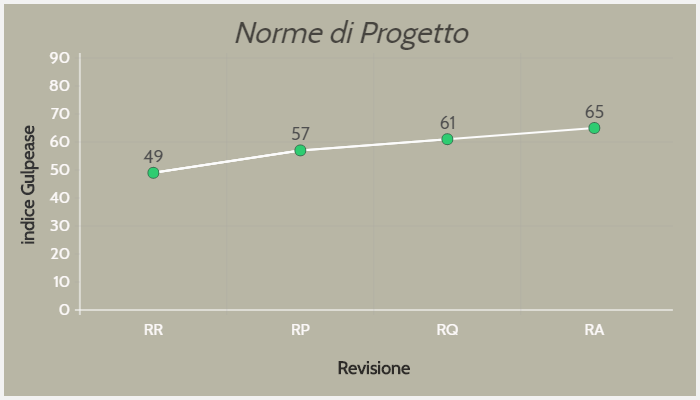
\includegraphics[scale=0.6]{includes/img/NdP.png}
	\caption{Miglioramento Norme di Progetto}
\end{figure}

